\documentclass[20pt]{extarticle}

% Large-print accommodation copy: bigger base font, single column, tighter
% (but still usable) answer space to avoid excessive page count.
\usepackage[top=0.3in, bottom=0.3in, left=0.35in, right=0.35in]{geometry}
\usepackage{tikz}
\usepackage{enumitem}
\usepackage{graphicx}
\usepackage{tgheros}
\renewcommand*{\familydefault}{\sfdefault}

\setlength{\parskip}{0pt}

% Change this value to resize the grade circle on the quiz header.
\newlength{\gradeCircleRadius}
\setlength{\gradeCircleRadius}{0.45in}

% Set this to the letter identifying this quiz version (e.g. A, B).
\newcommand{\quizVersion}{A}

\pagestyle{empty}

\begin{document}

\noindent
\begin{minipage}[t]{\dimexpr\textwidth-2\gradeCircleRadius-0.5in\relax}
    \textbf{ECGR 4101/5101 --- Advanced Embedded Systems}\par
    \textbf{Quiz 1: USB and CAN Bus --- Version \quizVersion\ (Large Print)}\\[6pt]
    Name: \makebox[2.3in]{\hrulefill} \quad Date: \makebox[1.4in]{\hrulefill}
\end{minipage}%
\hfill
\raisebox{0.15in}{%
\begin{minipage}[t]{\dimexpr 2\gradeCircleRadius+0.2in\relax}
    \centering
    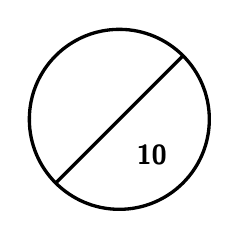
\begin{tikzpicture}[baseline=(circtop.base)]
        \coordinate (circtop) at (0,\gradeCircleRadius);
        \draw[very thick] (0,0) circle (\gradeCircleRadius);
        \draw[very thick] ({\gradeCircleRadius*cos(225)},{\gradeCircleRadius*sin(225)}) -- ({\gradeCircleRadius*cos(45)},{\gradeCircleRadius*sin(45)});
        \node at ({0.36*\gradeCircleRadius},{-0.4*\gradeCircleRadius}) {\textbf{10}};
    \end{tikzpicture}
\end{minipage}}

\vspace{0.05in}
\textit{For each question, circle the letter of the correct answer.}

\vspace{0.05in}

\begin{enumerate}[label=\textbf{\arabic*.}, leftmargin=*, itemsep=2pt]

\item \textbf{(5 points)} The figure below is a capture of the D+ and D- lines during a single \textbf{full-speed} USB data packet. The numbers along the top count the bit times, and each dotted line marks the boundary between two bit times.

\begin{center}
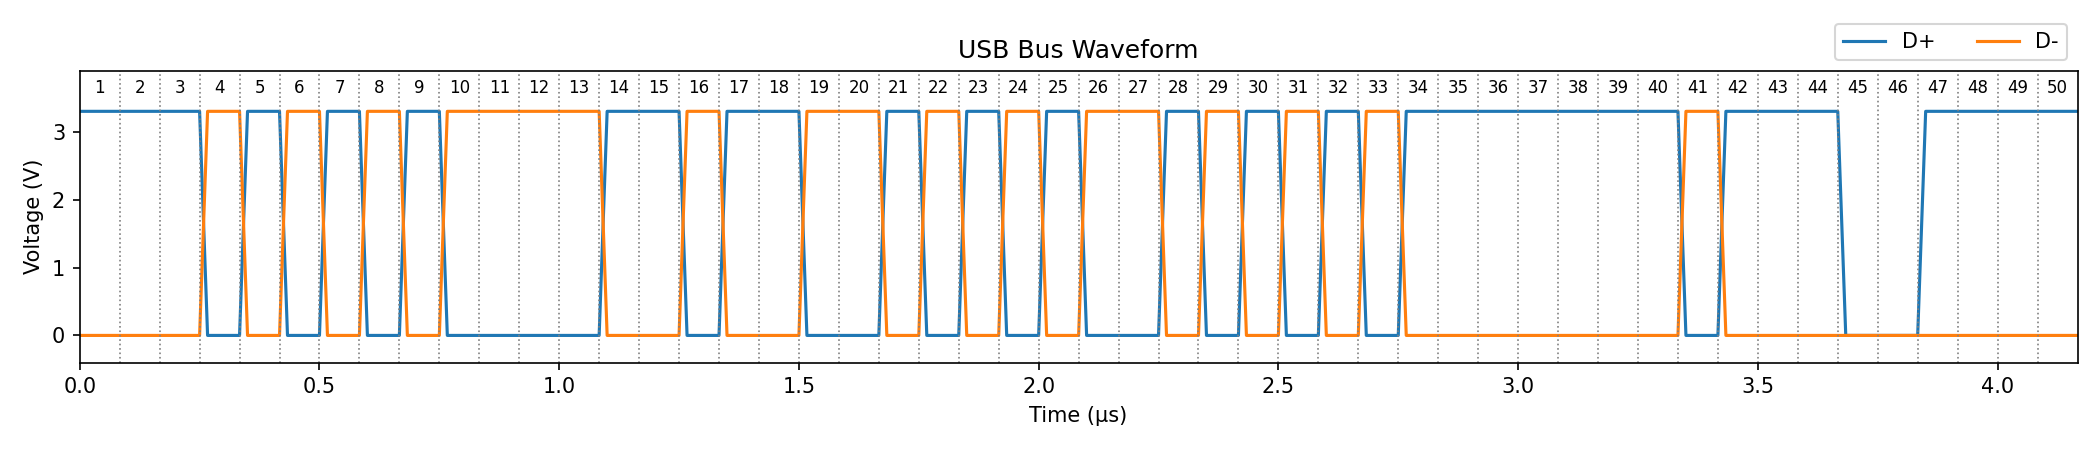
\includegraphics[width=\linewidth]{usb_waveform.png}
\end{center}

\begin{enumerate}[label=(\alph*), leftmargin=*, itemsep=6pt]
\item \textbf{(1 point)} Which bit times contain the \textbf{SYNC} field?

\begin{center}
\textbf{(A)} 1--3 \quad \textbf{(B)} 4--11

\textbf{(C)} 12--19 \quad \textbf{(D)} 20--27
\end{center}

\item \textbf{(1 point)} Which bit time(s) contain a bit-stuffing bit?

\begin{center}
\textbf{(A)} bit 34 \quad \textbf{(B)} bit 41

\textbf{(C)} bits 27 and 41 \quad \textbf{(D)} none
\end{center}
\end{enumerate}

\newpage

\begin{enumerate}[resume, label=(\alph*), leftmargin=*, itemsep=6pt]
\item \textbf{(3 points)} The PID field occupies bit times 12--19. Using NRZI decoding (a transition between consecutive bit times is a \texttt{0}; no transition is a \texttt{1}), decode these 8 bits and match them, LSB first, against the bus patterns below to identify the packet type.

\begin{center}
\begin{tabular}{ll}
\texttt{DATA0} & \texttt{11000011} \\
\texttt{DATA1} & \texttt{11010010} \\
\texttt{ACK} & \texttt{01001011} \\
\texttt{OUT token} & \texttt{10000111}
\end{tabular}
\end{center}

\begin{center}
\textbf{(A)} DATA0 \quad \textbf{(B)} DATA1

\textbf{(C)} ACK \quad \textbf{(D)} OUT token
\end{center}
\end{enumerate}

\newpage

\item \textbf{(5 points)} The figure below is a capture of the CAN\_H and CAN\_L lines during a single \textbf{standard frame} (11-bit identifier) CAN data frame. Recall that for CAN, a dominant bit is a logical \texttt{0} and a recessive bit is a logical \texttt{1}.

\begin{center}
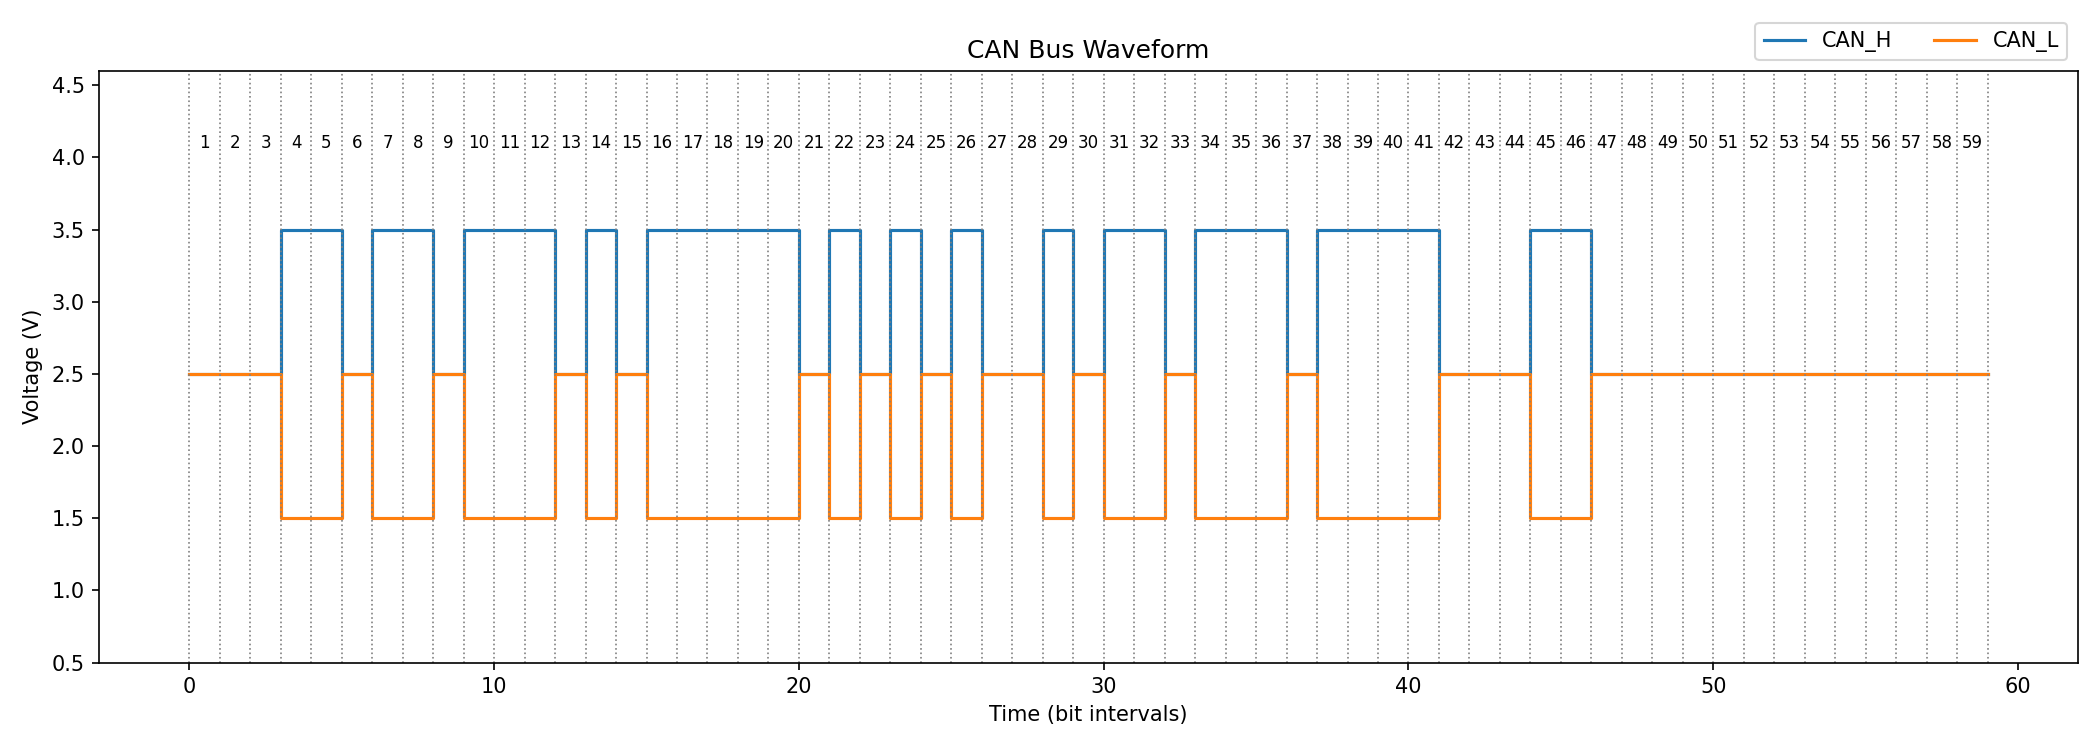
\includegraphics[width=\linewidth]{can_waveform.png}
\end{center}

\begin{enumerate}[label=(\alph*), leftmargin=*, itemsep=6pt]
\item \textbf{(1 point)} Which bit times contain the 11-bit \textbf{identifier} field, immediately following the Start-of-Frame (SOF) bit?

\begin{center}
\textbf{(A)} 1--3 \quad \textbf{(B)} 4--4

\textbf{(C)} 5--15 \quad \textbf{(D)} 16--26
\end{center}

\item \textbf{(1 point)} Which bit time(s) contain a bit-stuffing bit?

\begin{center}
\textbf{(A)} bit 14 \quad \textbf{(B)} bit 21

\textbf{(C)} bits 14 and 21 \quad \textbf{(D)} none
\end{center}
\end{enumerate}

\newpage

\begin{enumerate}[resume, label=(\alph*), leftmargin=*, itemsep=6pt]
\item \textbf{(1 point)} Based on the DLC field, how many data bytes does this frame carry?

\begin{center}
\textbf{(A)} 1 \quad \textbf{(B)} 2 \quad \textbf{(C)} 3 \quad \textbf{(D)} 4
\end{center}

\item \textbf{(1 point)} Decode the 11-bit identifier carried by this frame (bit times 5--15). Give your answer in hex.

\begin{center}
\textbf{(A)} 0x245 \quad \textbf{(B)} 0x244

\textbf{(C)} 0x645 \quad \textbf{(D)} 0x225
\end{center}

\item \textbf{(1 point)} If we have two identifiers that were transmitted at the same time, which one would be placed on the bus?

\begin{center}
\textbf{(A)} The identifier with the numerically lower value \quad \textbf{(B)} The identifier with the numerically higher value

\textbf{(C)} Whichever node started transmitting first \quad \textbf{(D)} Both are placed on the bus simultaneously
\end{center}
\end{enumerate}

\end{enumerate}

\end{document}
